\chapter{Preliminary Results}

\begin{figure}[h]
	\scalebox{0.6}{
	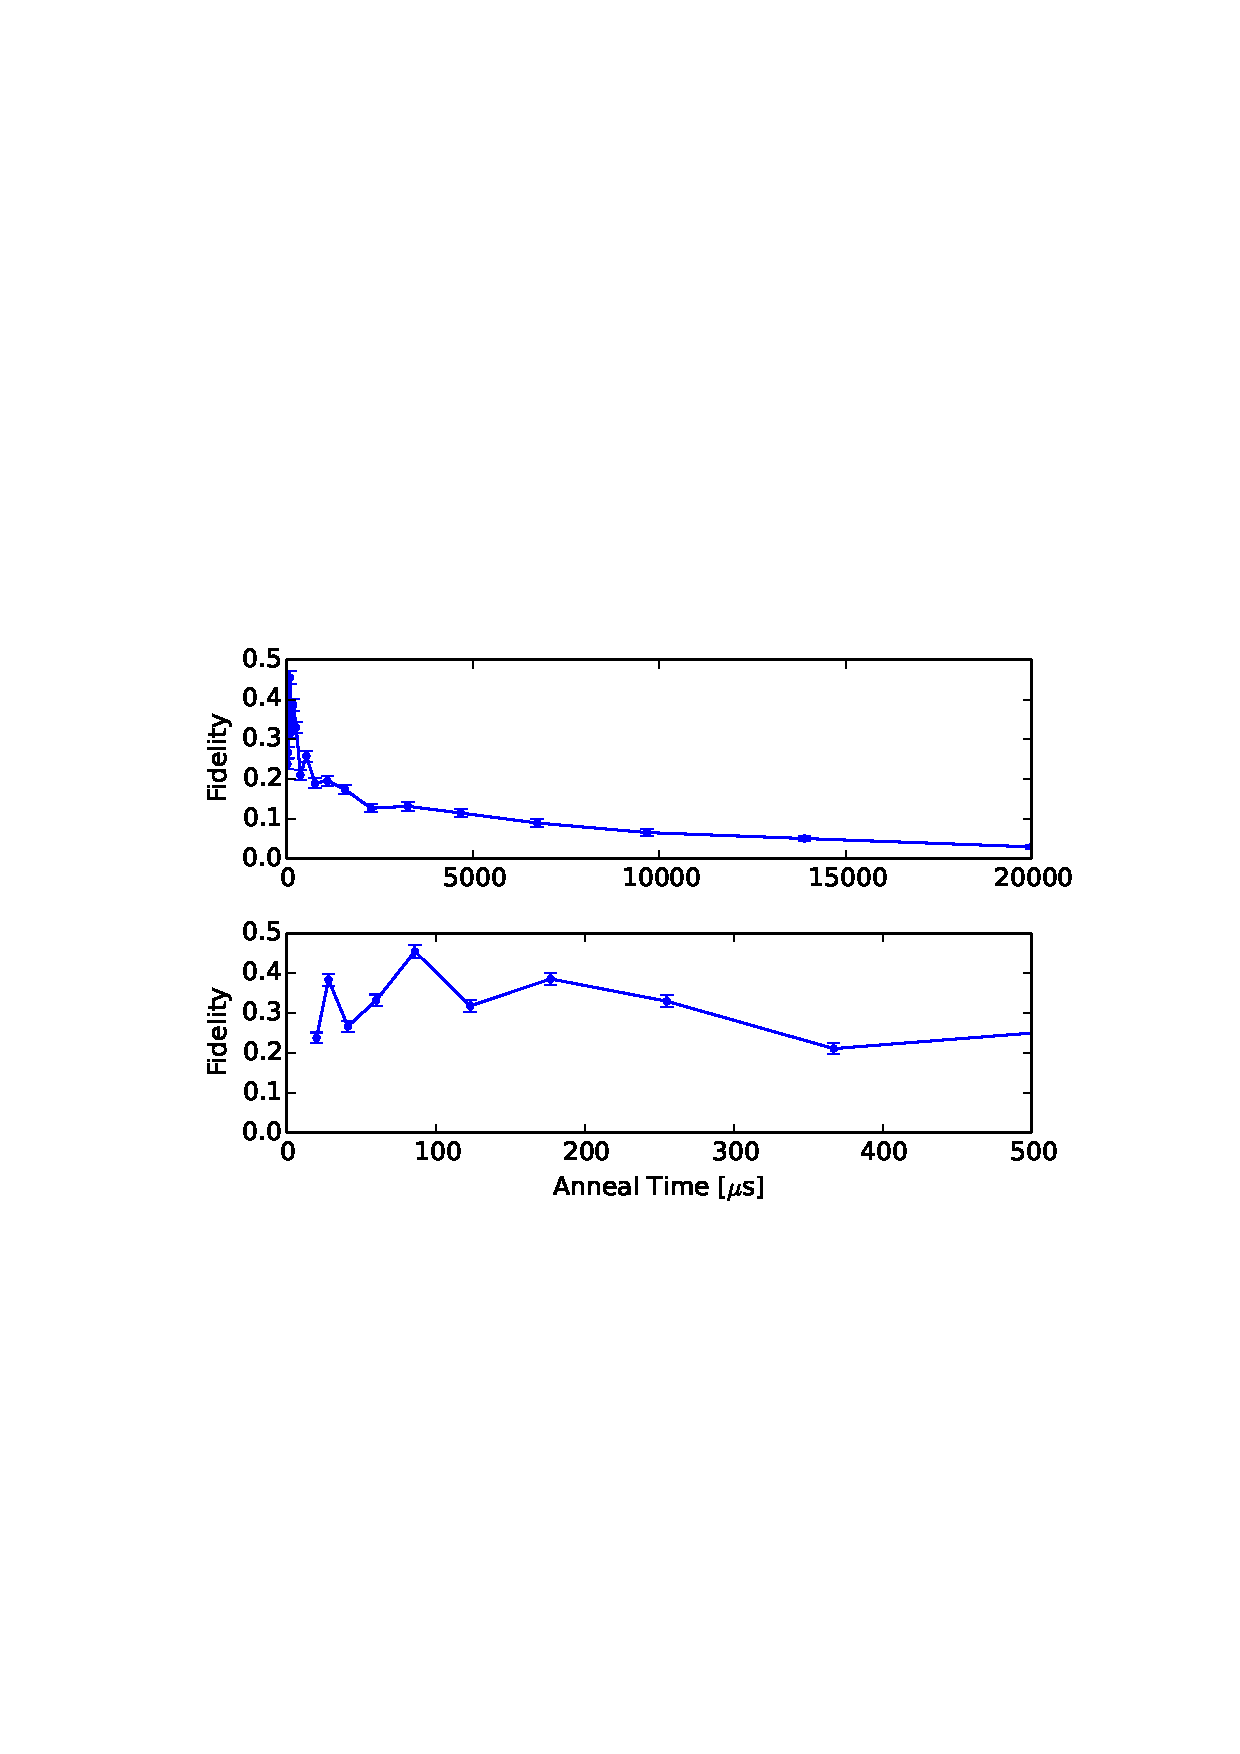
\includegraphics[bb=0 0 800 600]{img/6_018_2_fidelity.png}
}
	\caption[Fidelity vs Time]{Plot of the fidelity as a function of annealing time for the Hamiltonian ``6\_018'' both linear and log-scaled x-axis.}
	\label{fig:fidelity}
\end{figure}

Figure \ref{fig:fidelity} shows the results of 50,000 runs of the annealing machine consisting of 50 runs with 1000 reads at various annealing times.  Along the y-axis is the fidelity, and along the x-axis is the annealing time.  Contrary to what we expect from the adiabatic theorem and simulations of quantum annealing the fidelity is uncorrelated with annealing from 20$\mu$s out to roughly 500$ \mu$s, after which the fidelity \emph{decreases} with increasing annealing time.  This unexpected behaviour leaves us with a number of questions:

\begin{itemize}
	\item For short annealing times, why does the fidelity appear insensitive to annealing time?
	\item For long annealing times, why does the fidelity decrease with increasing annealing times?
	\item Is the short time fidelity dominated by the Hamiltonian programming noise?
	\item Is there significant drift in the fidelities after programming (i.e. read noise)?
	\item Does the Hamiltonian fidelity depend strongly on the number of coupling values?
\end{itemize}

or in short: Our theoretical model of quantum annealing suggests that the fidelity at T = 0 should be $2^{-N}$ for an $N$ spin Hamiltonian and increase as the annealing time increases, reaching approximately $1$ in the limit of $T \rightarrow \infty$ (as shown in Figure \ref{fig:simulated_anneal}).  Instead, the fidelity at our smallest accessible annealing time is already ``large'' and is seemingly insensitive to annealing time until the fidelity begins to \emph{drop} (as shown in Figure \ref{fig:fidelity}).

\emph{Why does the machine behave in this way contrary to our expectations?  Why does the short-anneal fidelity vary so much, and why does the long-anneal fidelity decrease rather than increase?}

\section{Short-time Evolution}
The data for short time evolution is inconsistent with the fidelity being a function of nothing but annealing time.  The fidelity between different runs varies significantly more than the standard deviation determined from averaging the reads.  Thus, there must be some other factor dominating the fidelity.  Options include:

\begin{itemize}
	\item Run noise in the machine: that is, each time the physical Hamiltonian is implemented the actual values of the fields and couplings are different, producing a different Hamiltonian every time.  This would mean that within a given run we see a consistent fidelity, but between runs we don't
	\item Our Hamiltonians might have too many coupling values, and resolution issues on the machine could be exacerbating the run noise
\end{itemize}

Our plan to resolve this question is to run smaller and simpler Hamiltonians until we can see smooth fidelity curves at small annealing times, or our Hamiltonians are so simple (i.e. 2-spin ferromagnetic ground states) that we are convinced the run noise is intrinsic.  By smaller and simpler, we mean (in order of increasing complexity):

\begin{itemize}
	\item Hamiltonians with no clones and \emph{no} couplings, only fields
	\item Hamiltonians with couplings lying in the range $\pm 1$
	\item Hamiltonians with clones
	\item Hamiltonians larger than a single k44
	\item Hamiltonians containing clone chains
\end{itemize}

\section{Long-time Evolution}
For a purely quantum system the fidelity should increase in the limit of increasing annealing time.  What we see instead in the actual data is that the fidelity appears to approach zero as the annealing time increases.  The physical computer is not an ideal quantum system, so to model it correctly we need to account for noise and decoherence sources.

We should fit this decreasing fidelity, or perhaps the population histogram, to some sort of model of thermal noise.  Then we could determine the energy leakage, maybe.







\begin{figure}
	\scalebox{0.35}{
		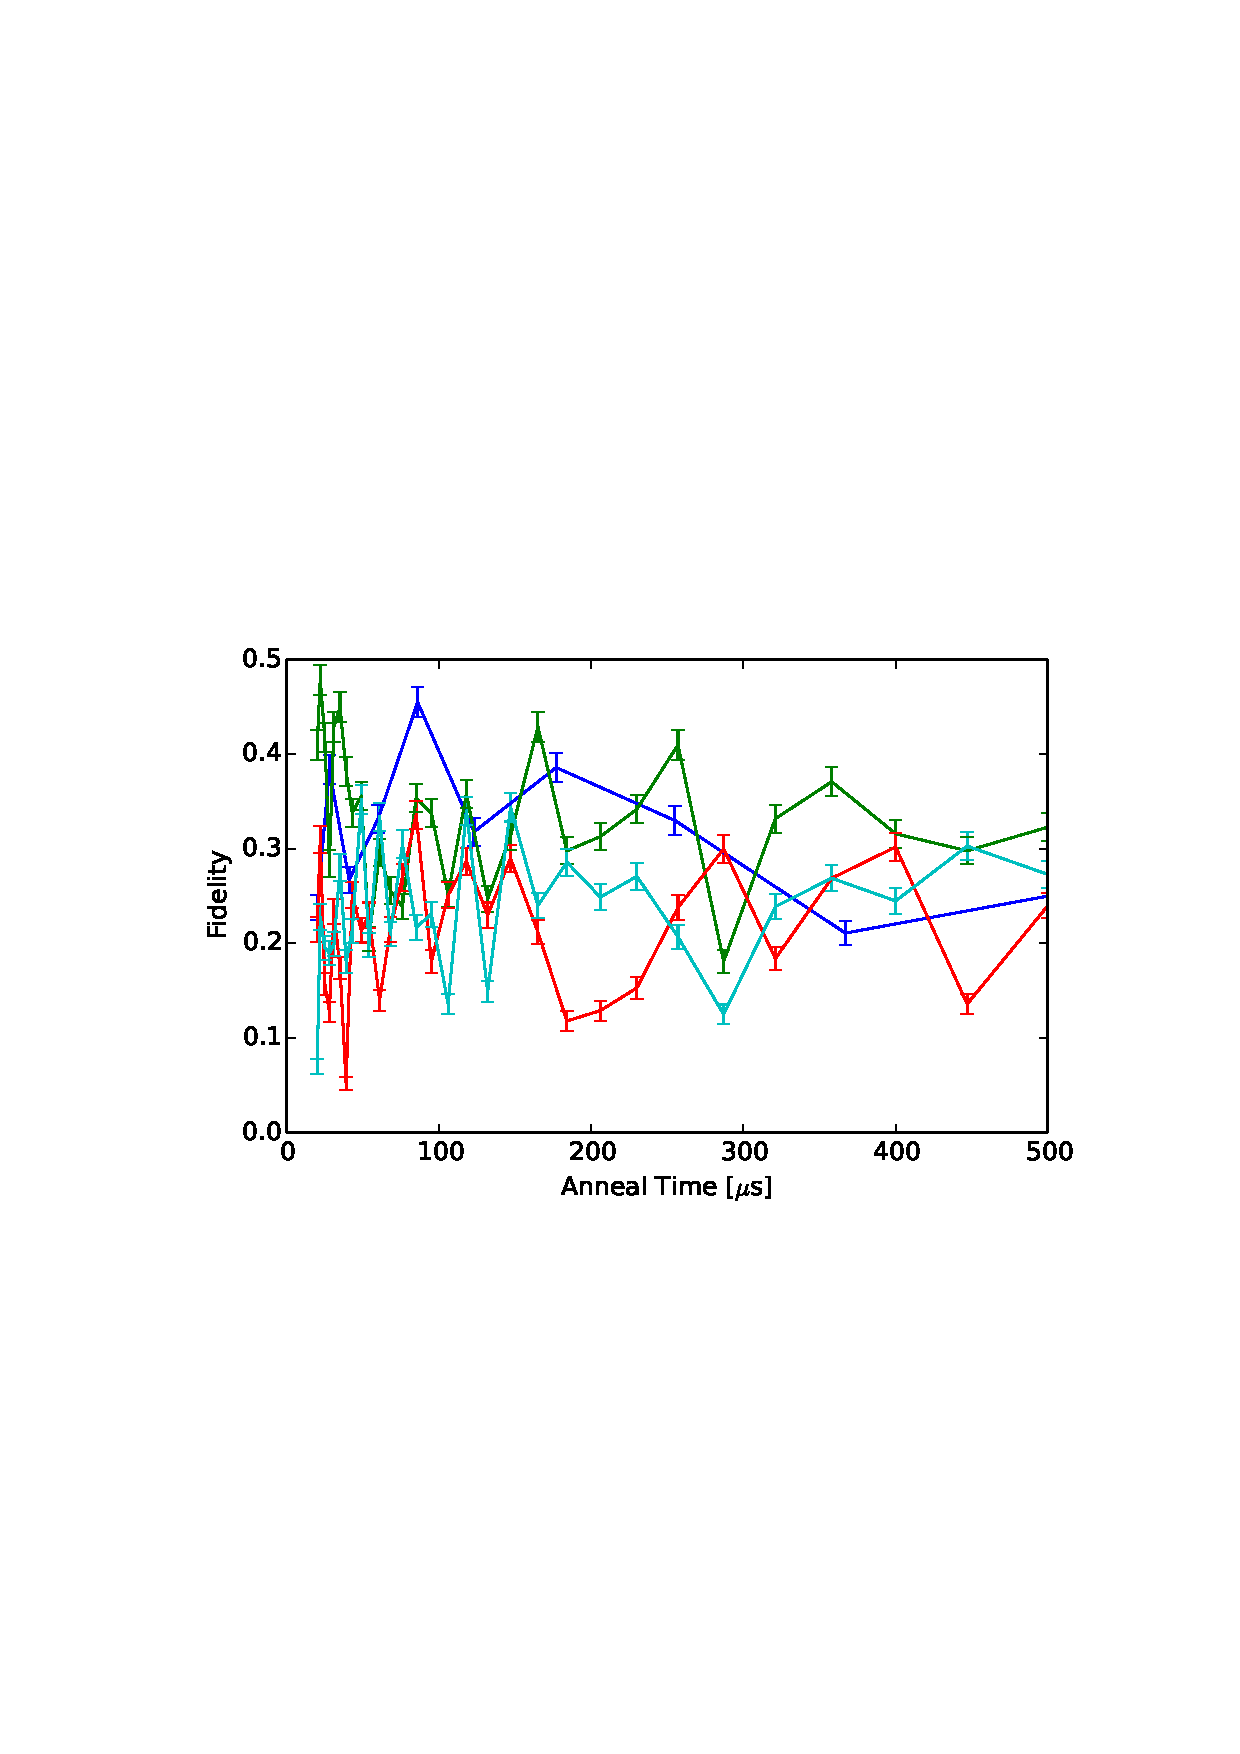
\includegraphics[bb= 0 0 745 382]{img/6_018_comparison.png}
	}
	\caption[Short Time Fidelities]{The fidelity as a function of time for the Hamiltonian ``6\_018'' for several different machine runs.  Each data point consist of 1000 machine reads.  Notice the spread between machine runs is outside of the error bars.}
	\label{fig:short_fidelity}
\end{figure}

\begin{figure}
	\scalebox{0.75}{
		\includegraphics[bb= 0 0 800 600]{img/4_5_hist.png}
	}
	\caption[Short Time Fidelity Histogram]{Histogram of the fidelities found for all annealing times  $< 500 \mu$s.  Notice the gaussian like structure.}
	\label{fig:fid_hist}
\end{figure}

\begin{figure}
	%\scalebox{0.75}{
	%	\includegraphics[]{}
	%}
	\caption[Simulation of Schr\"odinger's Equation]{Numerical integration of Schr\"odinger's Equation for the Hamiltonian ``k44'' showing the fidelity increasing to a plateau as the annealing time increases.}
	\label{fig:simulated_anneal}
\end{figure}

\begin{figure}
	%\scalebox{0.75}{
	%	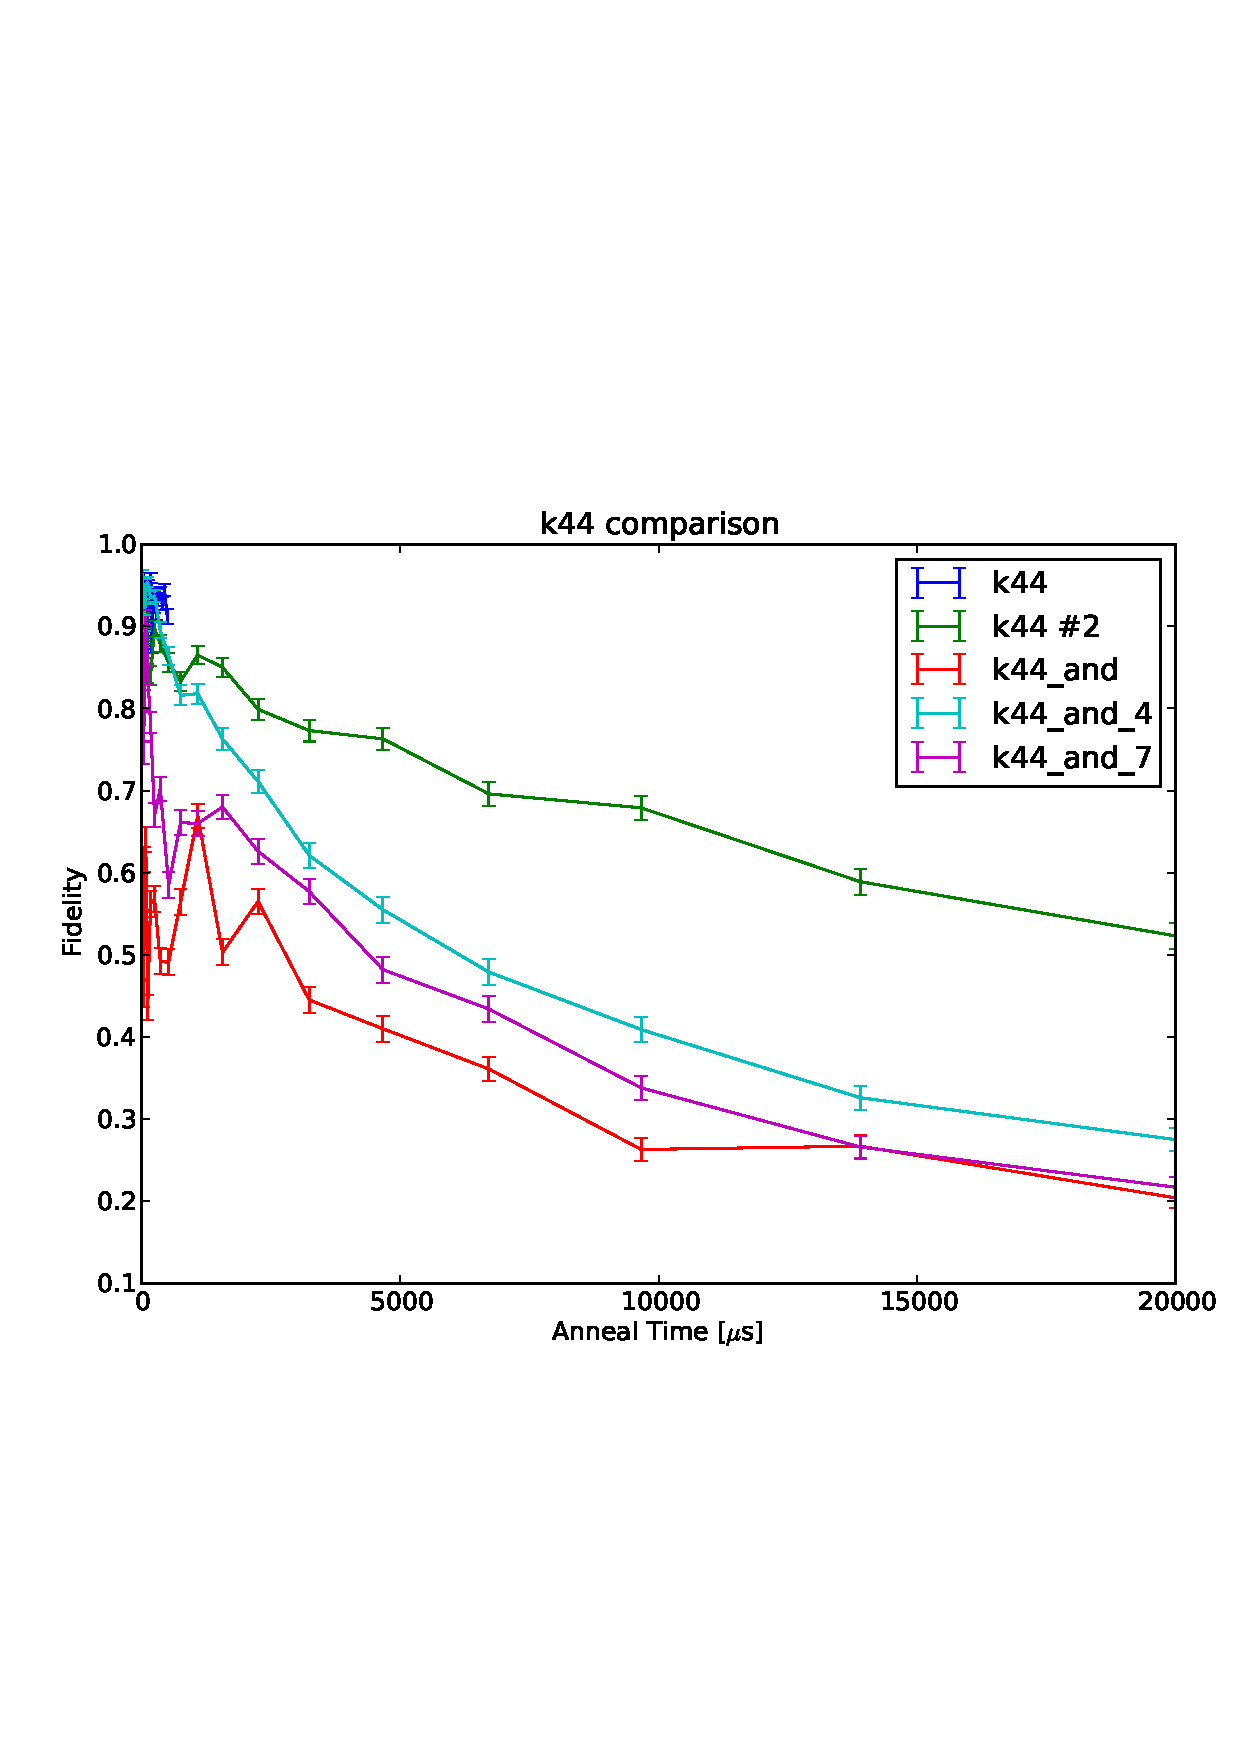
\includegraphics{img/k44_comparison.pdf}
	%}
	\caption[Long Time Anneal]{Machine data from Hamiltonian ``k44'' with 100 runs of 1000 reads showing the Hamiltonian noise at short times and the fidelity drop at long anneal times.}
	\label{fig:k44_long}
\end{figure}
